\documentclass{article}
\usepackage[utf8]{inputenc}
\usepackage{hyperref}

\title{Progress Report - Shamoon Siddiqui}
\author{Ghulam Rasool}
\date{May 2019}

\usepackage{natbib}
\usepackage{graphicx}
\usepackage{etoolbox}
\AtBeginEnvironment{quote}{\singlespace\vspace{-\topsep}\small}
\AtEndEnvironment{quote}{\vspace{-\topsep}\endsinglespace}

\begin{document}

\maketitle

\section*{Week 5/19/19 - 5/25/19}

\subsection*{Adversarial Learning in Statistical Classification: A
Comprehensive Review of Defenses Against Attacks\citep{miller2019adversarial}}

This was a thorough review of adversarial attacks and defenses. The basic story is that there have been several attacks and a handful of defenses developed. It seems that no single defense is robust against arbitrary attacks, so there's a shift towards anomaly detection (AD) instead of defending.
\newline\newline
Keywords: test-time evasion (TTE), data poisoning (DP), and reverse engineering (RE), anomaly detection (AD)

\section*{Week 5/26/19 - 6/1/19}
\subsection*{Adv-BNN: Improved Adversarial Defense through Robust Bayesian Neural Network\cite{liu2018adv}}

This work attempts to provide a defense against adversarial attacks by merging BNNs with adversarial training. Specifically, they note that Bayesian neural networks alone do NOT provide any defense against attacks. They discuss two accepted "standard" defenses: Adversarial training and Random Self Ensemble (RSE), which basically adds a noise layer at the inputs. This work utilizes \textit{Bayes by Backprop} to calculate the distributions for all of the weights. They experiment over the CIFAR-10, STL-10 and ImageNet143 datasets. The results are shown in Figure \ref{figure1}. They also note that adversarial training becomes intractable for higher dimension datasets.
\begin{figure}
    \centering
    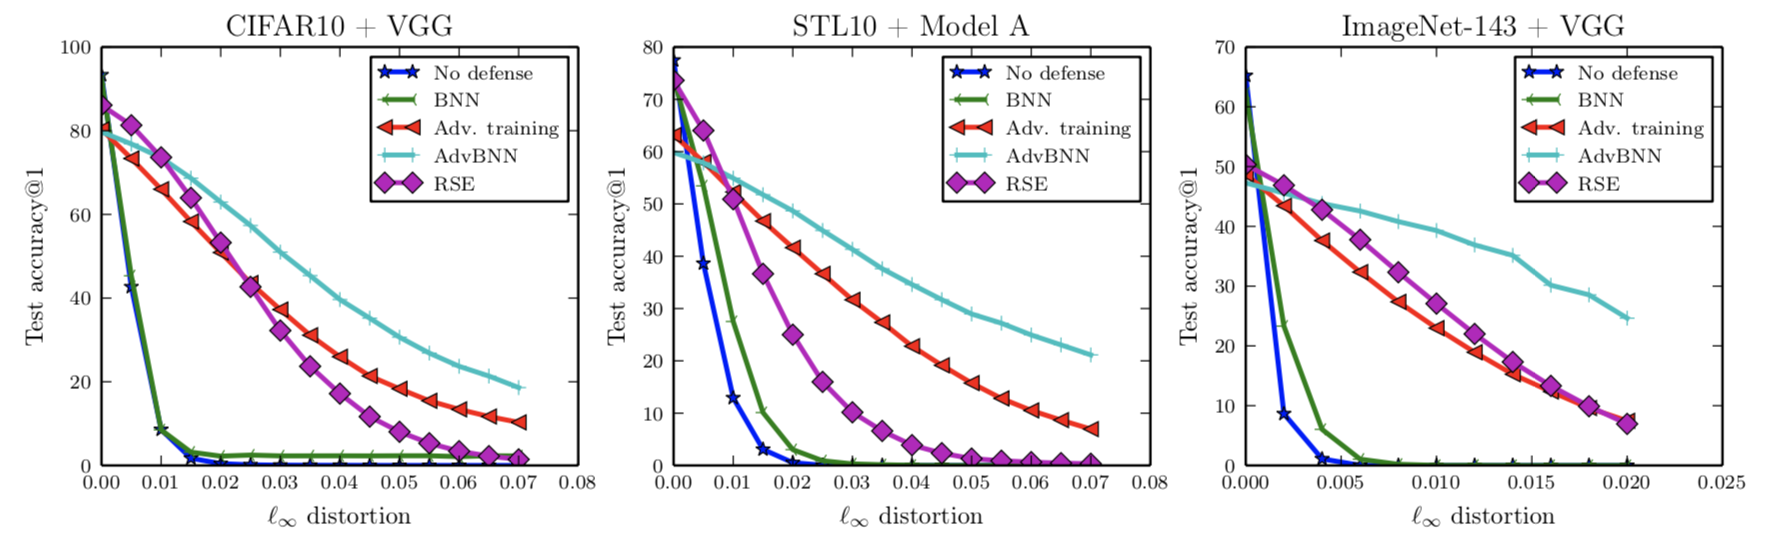
\includegraphics[width=1.0\textwidth]{results.png}
    \caption{Results for Adv-BNN}
    \label{figure1}
\end{figure}
\newline\newline
Keywords: bayesian neural network, adversarial training, bayes by backprop

\subsection*{Maybe Deep Neural Networks are the Best Choice for Modeling Source Code\cite{karampatsis2019maybe}}

This group presented a new neural language model for source code. The main problem with language models for source code is the \textit{out-of-vocabulary} (OOV) issue where new tokens are constantly being introduced at a rate that exceeds any natural languages. Must of this new tokenization is a result of never ending stream of developers and their idiocynracies, internal company coding standards and copy/pasting from online sources. The authors present a "subword token" model, in which they create tokens to be subwords (pretty obvious, I'd say). This allows them to handle newly seen vocabulary that was not in the initial training corpora. They use \textit{byte pair encoding} BPE to merge smaller tokens into larger ones. They also, at this time, have the most tokens (over 1 billion) which is 100x larger than any previous work.
\newline\newline
Keywords: neural code generation, n-gram models, neologism, out-of-vocabulary

\section*{Week 6/2/19 - 6/8/19}
\subsection*{Novelty search and the problem with objectives (2011)\cite{lehman2011novelty}}

Evolutionary Algorithms (EA) typically have some sort of a fitness, or objective function. This paper presents a method of "non objective search," in which an algorithm does not try to maximize some reward or minimize a cost. Rather, it uses novelty as a proxy for stepping stones. Specifically, the algorithm rewards instances that are functionally different from whatever was tried before. The analogy here is that of a robot trying to escape a room. Rather than giving it an objective of finding the door, opening the door, navigating objects, etc, it learns by novel behavior. Once it's explored every part of the room, it needs to find a new novel thing to do - such as turning a doorknob. This is similar to curiosity seeking in Reinforcement Learning. The goal they were trying to achieve in their experiment is a maze solving machine. As in all papers, they show their method scales better to complex maze problems.
\newline\newline
Keywords: genetic algorithm, evolutionary algorithm

\subsection*{Adversarial reprogramming of neural networks (2018)\cite{elsayed2018adversarial}}

Here, the authors describe a new form of attack. Rather than perturbing a few pixels to fool a classifier, they a model is repurposed to perform a new task. We assume an adversary has access to the parameters of a neural network and they want to reprogram the model. The reprogramming should perform a new task - by crafting an adversarial program to be included in the network input. As a concrete example, consider an Inception V3 ImageNet model. Using their methodology, it can be repurposed to function as an MNIST classifier, or a CIFAR-10 classifier.

The important takeaways here are that we don't need to be limited in thinking about attacks as pixel changes. There is a lot more interesting work going on in crafting new attacks.
\newline\newline
Keywords: adversarial learning, new attacks, imagenet, cifar-10, mnist

\subsection*{code2seq: Generating sequences from structured representations of code (2018)\cite{alon2018code2seq}}

The key innovation here is that instead of using words and sentences, they seem to convert the source code to an abstract syntax tree (AST). I don't fully understand attention, but they use attention to weight the various paths of the abstract syntax tree. The work is done on the Java programming language and the tasks they have are: code summarizing, code captioning (from StackOverflow data), and code documentation.

Of course, they achieve SOTA in all of these tasks.
\newline\newline
Keywords: neural code translation, abstract syntax trees, neural machine translation


\section*{Week 6/9/19 - 6/16/19}
\subsection*{Spell once, summon anywhere: A two-level open-vocabulary language model (2018)\cite{mielke2018spell}}

Most generative language models use word-level tokenization, but Out-of-Vocabulary tokens present an issue. Character level tokenization has an issue that it can't look back very far. The authors proposed 2 RNN's to solve this dichotomy by having one solve for context, with the other solving for character level spelling. I am unsure if it's end-to-end trained, but I'd like to spend more time to find out. For comparisons, they use a pure character-level RNN, which performs poorly, pure byte-pair encoding, which performs reasonably well.

They note that for frequently occuring words, all models do a reasonable job, but for rare words, the PURe-BPE and their model perform best. As for test dataset, they use WikiText-2 and the Multilingual Wikipedia Corpus.
\newline\newline
Keywords: rnn, word-level, char-level, ensemble

\subsection*{On the Convergence and Robustness of Adversarial Training (2019)\cite{wang2019convergence}}

The short story here is that when doing adversarial training, start with the easy examples in the beginning phases of training and increase difficulty of the adversarial examples as the training progresses. They posit that adversarial training is currently state of the art and their "dyanamic training strategy" outperforms existing methods.

To quantify "easy" vs" hard," they devise a new criterion dubbed a First-Order Stationary Condition for constrained optimization (FOSC). They show that this is a valid criterion to judge convergence of the inner loop of the min-max optimization.
\newline\newline
Keywords: adversarial training, optimization, min-max

\subsection*{A study of the uniqueness of source code (2010)\cite{gabel2010study}}

Great paper that goes into uniqueness. The question they pose is a thought experiment:
\newline
\begin{quote}
You are a software engineer starting a new project, requirements in hand. Unfortunately, your keyboard has malfunctioned, and your only method for entering program text is through copying and pasting existing code fragments. Fortunately (perhaps), you have oracle-like access to all source code that has ever been written. How much can you accomplish?
\end{quote}
They consider source code as being comprised of smaller units of source code and they attempt to model experiments to calculate syntactic redundancy. Most interestingly, they retokenize by replacing variable names with some sort of identifier on a per file basis. That part is pretty clever, for sure.
\newline\newline
Keywords: statistical code summarization, thought experiment, source code

\subsection*{Summarizing Git Commits and GitHub Pull Requests Using Sequence to Sequence Neural Attention Models (2017)\cite{zaidi2017summarizing}}}

This is not a published paper, per se, but seems to be a Master's project or some other class project. Nonetheless, I think it is an interesting idea so I added it to my reading list. The idea is (as suggested by the title) to take diffs from Github and translate it to a pull request message.

Their training data is massive, almost 350 GB, so they don't load it in memory, but rather use Azure Storage. They then filter only active repositories (one committer and separate reviewer in the past 6 months and pull request messages with at least 20 characters).

They restrict their languages to: Python, Ruby, Java, Javascript, R, Scala and C#. Their model is a standard sequence-to-sequence attention model. Since a git commit is a series of add / remove lines, they append a <DEL> or <ADD> token to the beginning of the line.

When it comes to evaluation, there are no standard benchmarks (kudos to them for setting one!) so they use cosine-similarity to calculat a BLUE score to get average n-gram precision.
\newline\newline
Keywords: neural code translation, github, sequence-to-sequence, attention

\section*{Week 6/17/19 - 6/23/19}
\subsection*{Modeling Vocabulary for Big Code Machine Learning (2019)\cite{babii2019modeling}}

This paper is a survey of a variety of methods to tokenize a corpus of source code. They compare the methods by vocabulary size and tokens. Although not the primary focus on the paper, they also check training times against a code completion task.

The problem is that, "While software is more repetitive than natural language, software vocabulary is much more diverse as developers can create new identifiers at will." This leads to a never ending class of Out-of-vocabulary problems. Several methods are studied in this paper to establish some baselines: unsplit, word splitting and byte-pair encoding (BPE). As expected, BPE has the most significant gains by reducing the vocabulary size 1,000x. "We conclude that as a rule of thumb, a BPE with a 1–2\% token increase performs very well."

During training, they configured LSTM's with layer size of 300, 650 hidden units and 3 LSTM layers. Furthermore, all of their training was done on a consumer grade Geforce GTX 1080. Their fastest model can process one epoch (1.1m files) in ~ 6 hours.

Conclusion: BPE is the way to go with neural code tasks.
\newline\newline
Keywords: embeddings, word2vec, byte-pair-encoding, code completion, survey



\section*{Week X/XX/19 - X/XX/19}
\subsection*{Paper Title (Year)\cite{miller2019adversarial}}

Things I want to talk about.
\newline\newline
Keywords: keyword, list


\bibliographystyle{plain}
\bibliography{references}
\end{document}
